\documentclass[a4paper,10pt]{article}
\usepackage[a4paper,portrait]{geometry}

\setlength{\textheight}{24.5cm}
\setlength{\textwidth}{16.5cm}
\addtolength{\rightmargin}{-1cm}


\usepackage[usenames,dvipsnames]{color}
\usepackage{colortbl}
\usepackage{graphicx}

\usepackage{hyperref}

\hypersetup{
pdfauthor   = {Angela Lucaci-Timoce <angela.isabela.lucaci.timoce@cern.ch>},
pdftitle    = {WHCAL},
pdfsubject  = {WHCAL},
pdfkeywords = {CALICE},
pdfcreator  = {LaTeX with hyperref package},
pdfproducer = {dvips + ps2pdf},
colorlinks  =true,  %%% links are colored
urlcolor    =Blue,  %%% color of external links
citecolor   =Blue,
breaklinks  =true,  %%%allow links to break over lines (default:%%%false).
bookmarks   =true,
%bookmarksdepth =false,
unicode     =true, %%%create Unicode bookmarks
pdfpagemode ={UseOutlines}%%%UseOutlines, FullScreen
}

%%=======================================================
\definecolor{myPaleYellow}{RGB}{255,250,205}

%%=======================================================

%opening

\title{ {\normalsize LCD-Note-2011-001 \\ \vspace{5mm}}
{Temperature studies of the CALICE W-HCAL \\ with CERN 2010 data}}
\author{Dominik Dannheim, Wolfgang Klempt, Angela Lucaci-Timoce}

%=============================================================
\begin{document}

\maketitle

%\begin{abstract}
%\end{abstract}

%=============================================================
\section{Temperature measurement and correction}
\subsection{Temperature dependence of SiPM properties and correction strategy}
The properties of the Silicon Photomultipliers used for the readout of the A-HCAL prototype changes 
with temperature \cite{niels-diplomarbeit}:
\begin{itemize}
\item \emph{Gain}:  The gain $G$ of the SiPMs decreases with 1.7\%/K with increasing temperature. 

\item \emph{Response}: The response $A^{MIP}$ decreases with 3.7\%/K with increasing temperature. 

\item \emph{Breakdown voltage}: The breakdown voltage $U_{bd}$ increases by 65~mV/K with increasing temperature.
\end{itemize}

The temperature-dependence of all other elements of the readout chain is expected to be negligible
compared to the one of the SiPMs. 

To be able to correct for the temperature-induced change of the SiPM properties, a continous monitoring
of the SiPM temperatures is performed. All calibration and physics data is normalised per readout cell
to the average temperature at which the MIP scale has been determined for the respective cell. Note that with
this correction scheme a global constant offset in the temperature scale does not affect the obtained results,
as only relative differences enter the calculations.

\subsection{Temperature monitoring during data taking}
The temperatures inside the readout layers are monitored continously using a set of five
integrated precision temperature sensors LM35~\cite{temp-sensors} per module. The accuracy
of the sensors is guaranteed to be at the level of 0.5$^o$C. The typical nonlinearity is $\pm$0.25$^o$. 
The sensor output voltage increases linearly with 10.0~mV/$^o$C. The signals from all 5 sensors in one
module are multiplexed and read out through a common ADC~\cite{sven-karstensen-private}. 
A hardware offset calibration was performed after assembly, to correct for  
voltage drops in the cables and the offsets
of the ADC. Remaining systematic shifts in the absolute temperature scales are accounted for with a 
calibration procedure described in section~\ref{offset-determination}. 

The configuration of the sensors inside
the modules is shown in Fig. \ref{sensor-config}. The sensors for module 1 and 2 (installed in layers 29 and 30,
respectively)
are mounted in a diagonal configuration from top right to bottom left (looking into the direction from where
the beam originates).  The sensors for modules 3 to
30 (layers 1 to 28) are mounted in a vertical configuration from middle top to middle bottom. 
Each readout cell is assigned to one temperature sensor, based on its vertical distance to the respective 
sensor, as indicated in the figure.
The temperature for each readout cell is approximated as the temperature measured by the sensor assigned
to it, without further interpolation or averaging. 

\begin{figure*}[t]
\label{sensor-config}
\centering
\includegraphics[width=15cm]{sensor-config.pdf}
\caption{Approximate position of the temperature sensors inside the A-HCAL readout modules. The dashed
red circles labeled 1a to 5a represent the positions for modules 1 and 2 (layers 29 and 30). The solid blue circles
labeled 1 to 5 represent the positions for modules 3 to 30 (layers 1 to 28). The assignment of readout cells
to temperature sensors is indicated with dashed magenta lines representing the division between neighbouring
sensors.}
\end{figure*}

During data taking, a set of temperature measurements is performed approximately every 6 minutes and saved
to a database. The temperature values stored in the data base are used offline to correct for the 
temperature-induced change of the SiPM properties. 

The muon runs used to determine the MIP scales have been taken over several weeks in the 
T7 beamline of the CERN PS in September/October 2011 (runs 360114 until 360306). 
The average temperature of all modules during
 these runs was measured to be 24.6$^o$C, with a spread of approximately $\pm$2$^o$C.

Physics and calibration runs have been taken within 
two weeks in the T9 beamline of the CERN PS in November 2011 (runs 360366 until 360870).
 The average temperature of all modules during these runs was measured to be between 
approximately 19$^o$C and 26$^o$C, with an average of
21.8$^o$C.

\subsection{Determination of calibration offsets}
\label{offset-determination}
\subsubsection{Measurement principle}
To improve the accuracy of the temperature measurements, a calibration procedure is applied to remove
systematic offsets from the measured temperature values of each sensor. The calibration measurement 
requires all sensors to be at the same reference temperature $T_{ref}$, measured externally with 
high precision.  For each 
sensor $i$ , the temperature offset $o_{i}$ is determined as the difference between the 
measured raw temperature $T_{i,calib}$ and $T_{ref}$:
$$o_i=T_{i,calib}-T_{ref}$$
We assume that the offset is both stable over time and over the range of observed temperatures in the
testbeam setup. The true temperature $T_i$ for each sensor is thus given by its measured raw temperature 
$T_{i,raw}$ and the previously determined offset $o_i$: 
$$T_{i}=T_{i,raw}-o_i$$

The offsets determined from the calibration measurement are subtracted from the measured raw temperatures
by the PVSS script that writes the temperatures to the database. 

\subsubsection{Offset measurements for the CERN 2010 configuration}

For all runs before 360829, old temperature
offsets from a Fermilab testbeam campaign in 2008 (FNAL 2008 offsets) 
have been used to calculate the temperatures written 
to the database. For all runs including and after 360829, all offsets were set to zero. A new calibration
of the temperature offsets for the CERN 2010 configuration has only been performed in February 2011, 
when the A-HCAL prototype was installed again in the T7 testbeam area of the CERN PS. 
In order to apply the offsets determined with this calibration, the offline treatment of the
temperatures in the database was changed as described in section~\ref{offline-implementation}.

Calibration offsets for the CERN 2010 configuration have been determined with temperature readouts
of the cold calorimeter, immediately after switching on the LV power supplies and enabling the
crate-monitoring boards.
The reference temperature $T_{ref}$ is measured at the back 
face of the calorimeter stack with two NT100 temperature probes attached to the outside of layer 30.
The accuracy of this measurement was estimated to be approximately $\pm0.5^o$C.  It was found that 
the day-night temperature fluctuations in the T7 area of approximately $\pm2^o$C 
in connection with the large heat capacity of the tungsten stack
lead to an inhomogenous distribution of the raw temperature measurements over the layers. When measuring
in the morning, after the temperature in T7 had decreased over night, the inner layers showed significantly
higher temperature offsets by approximately $1^o$C than the outer layers. Figure \ref{fig-offsets-largespreads} 
shows the distribution of the temperature offsets over the layers (left) and of the average temperatures per layer (right)
for one measurement in such instable temperature conditions.  The offsets for layer 19 (module 21) sensor 5 and
for layer 29 (module 1) sensor 1 are excluded from the plots, as those sensors are permanently malfunctioning and 
have no sensible readout values.

The offset measurements have been repeated over several days with varying atmospheric conditions until 
a period of only small day-night temperature fluctuations of approximately $\pm$0.5$^o$C was reached. 
The resulting
offsets in these conditions show smaller systematic variations between inner and outer layers of $<0.5^o$C,
as shown for one example in Fig.~\ref{fig-offsets-smallspreads}. The offsets from this measurement have been
selected to be applied to all CERN 2010 temperature measurements (CERN 2010 offsets).

\begin{figure*}[t]
\label{fig-offsets-largespreads}
\centering
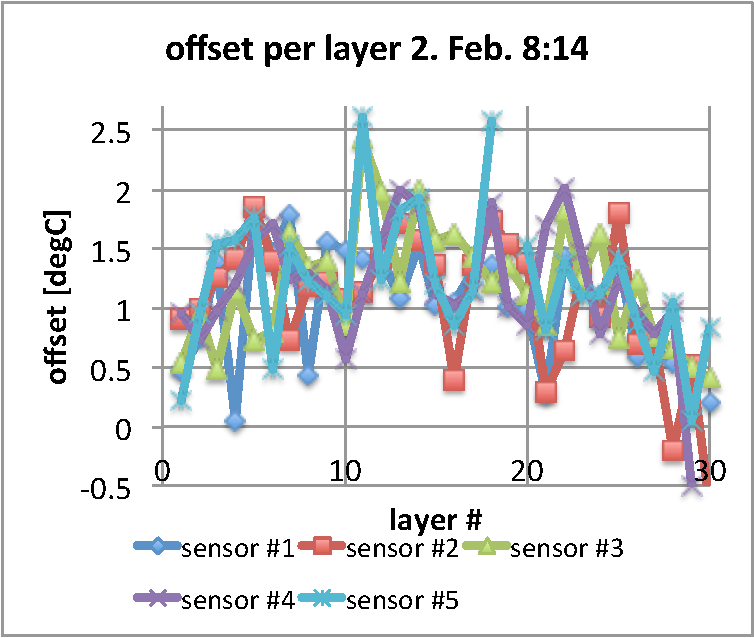
\includegraphics[width=8cm]{offset-per-layer-2-feb-8_14.pdf}
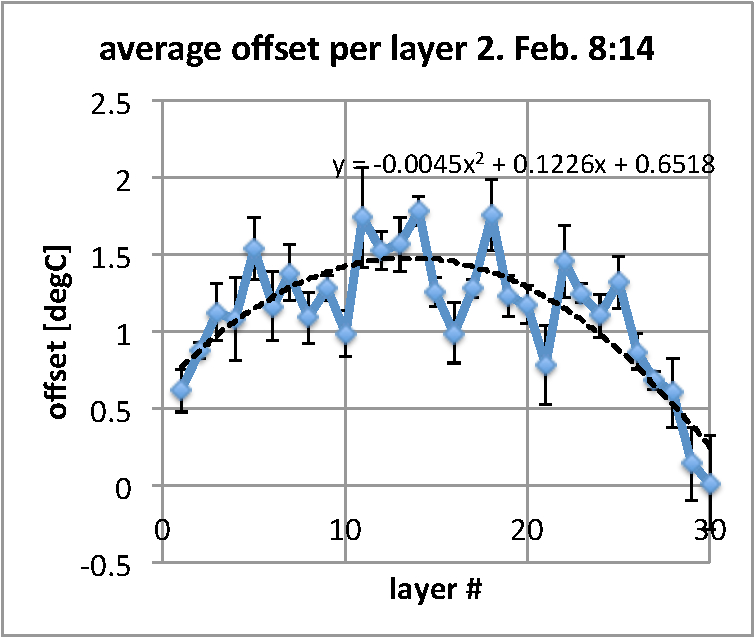
\includegraphics[width=8cm]{average-offset-per-layer-2-feb-8_14.pdf}
\caption{Temperature offsets measured after a cold night on the morning of February 2nd (left), 
as well as averages per layer
and standard deviations for the same measurement (right). 
The dashed line represents a quadratic fit to the data.}
\end{figure*}

\begin{figure*}[t]
\label{fig-offsets-smallspreads}
\centering
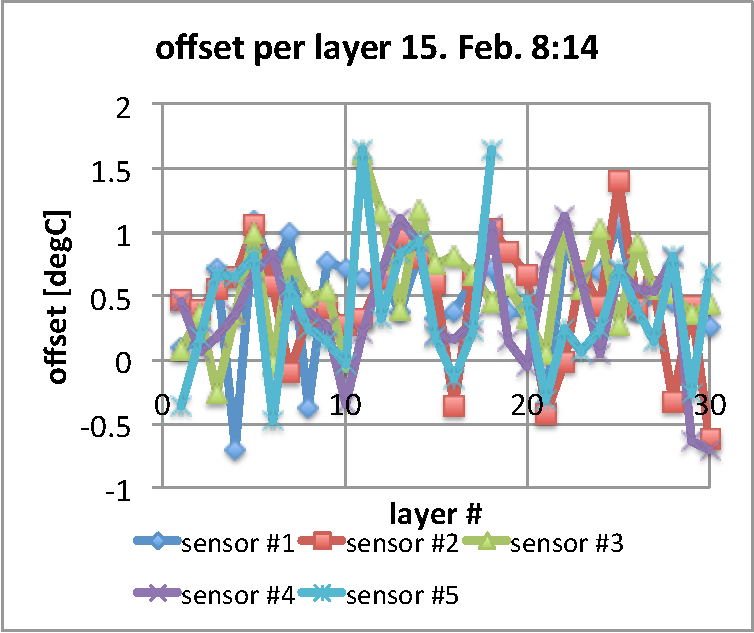
\includegraphics[width=8cm]{offset-per-layer-15-feb-8_48.pdf}
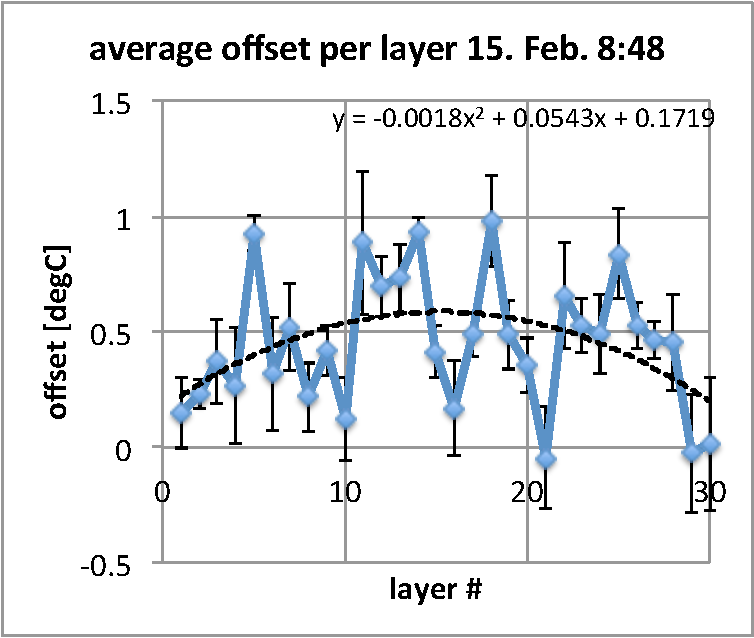
\includegraphics[width=8cm]{average-offset-per-layer-15-feb-8_48.pdf}
\caption{Temperature offsets measured in stable outside temperature conditions
on February 15th (left), as well as averages per layer
and standard deviations for the same measurement (right). 
The dashed line represents a quadratic fit to the data.}
\end{figure*}

\subsection{Temperature profiles in physics runs}
The temperature offsets described above have been applied to temperature measurements during
physics runs and compared to the FNAL 2008 offsets as well as to the raw temperature measurements.
Figure~\ref{fig-temp-profiles-run360829} shows the resulting temperature profiles for one example (first 
temperature measurement in run 360829). As expected, the raw-temperature profile shows a larger spread
than the ones with offsets applied. The profile with FNAL 2008 offsets shows still a rather large spread
and a systematic shift by -4$^o$C. This systematic shift is likely to be due to an inaccurate determination
of the reference temperature during the offset measurement at FNAL in 2008~\cite{sven-karstensen-private}.   
The new offsets determined at CERN result in a smaller spread of the temperature profile. With these offsets
applied, the spread in temperatures per layer becomes larger for larger layer numbers. A possible explanation
for this trend could be the presence of additional heat sources (test equipment from alternative readout concepts)
under the last layers of the calorimeter stack and/or a different configuration of cooling fans in this region.
 
\begin{figure*}[t]
\label{fig-temp-profiles-run360829}
\centering
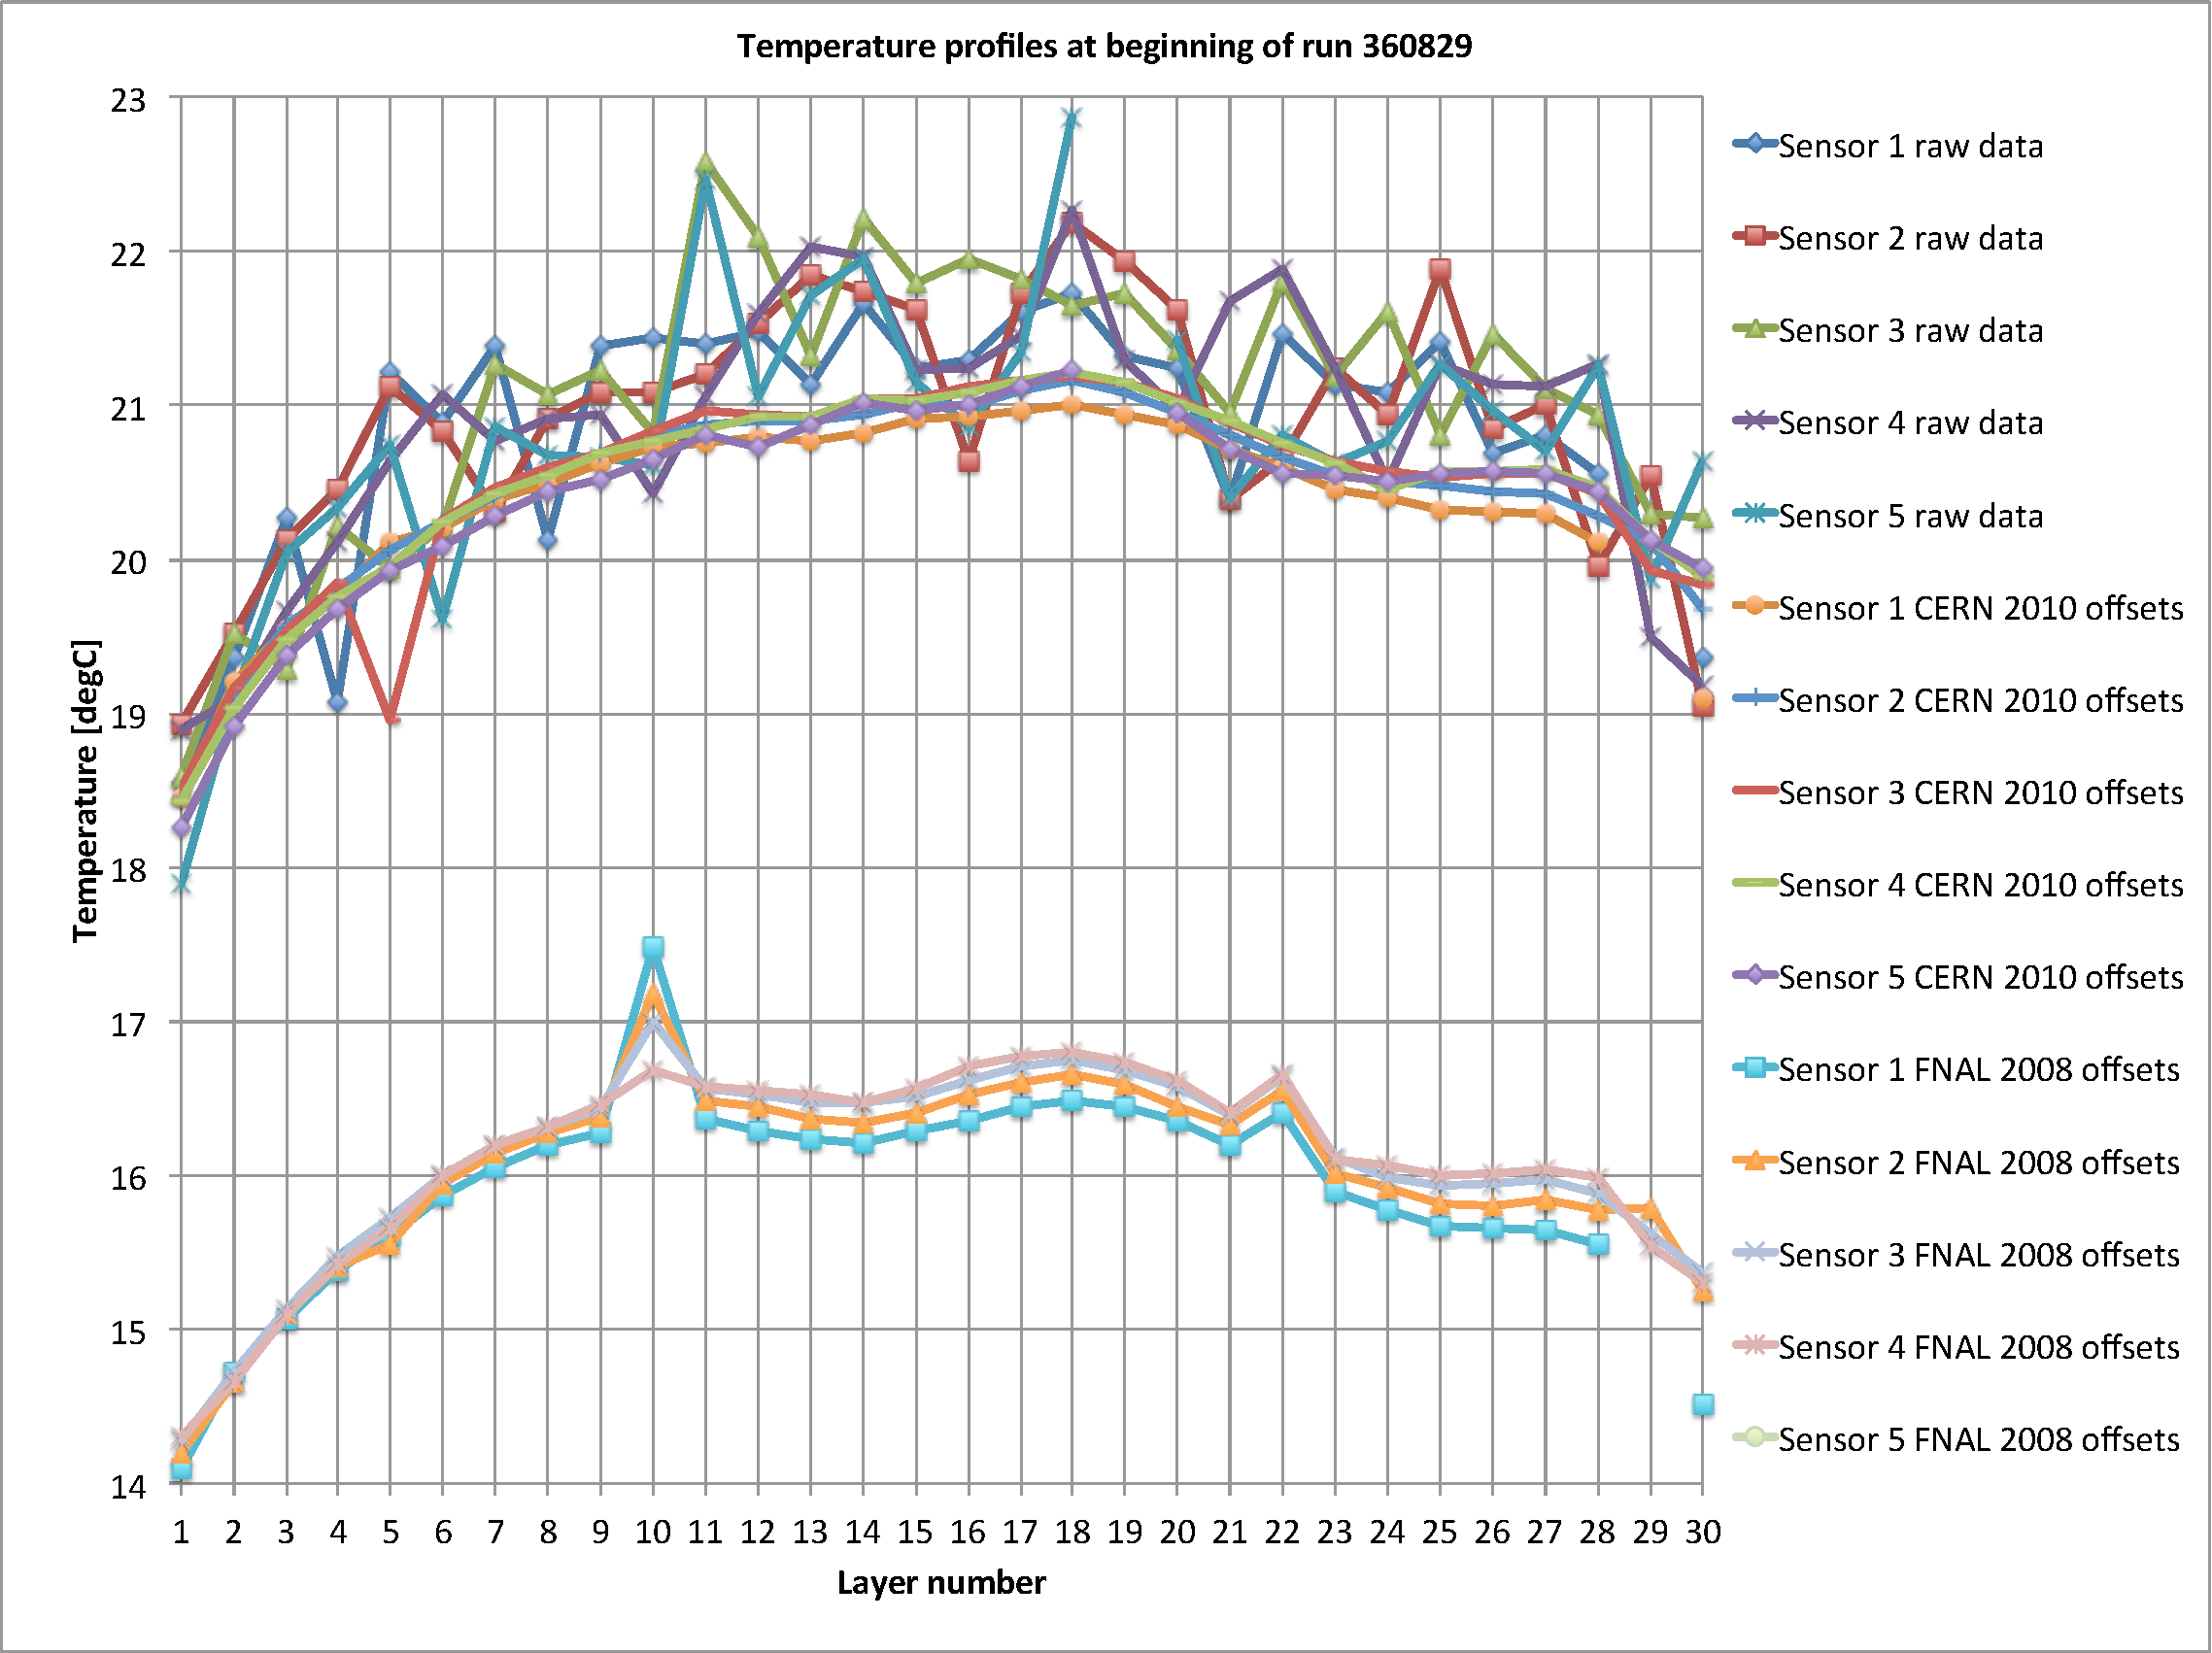
\includegraphics[width=16cm]{temp-profiles-run360829.pdf}
\caption{Temperature profiles for the first temperature readout in 
physics run 360829. The raw temperature data is compared to temperature
data obtained with the old FNAL 2008 offsets and with the new CERN 2010 offsets.}
\end{figure*}


%=============================================================
%=============================================================
%=============================================================
%=============================================================
\section{Implementation of the temperature related issues in the CALICE software}
\label{offline-implementation}
%=============================================================
\subsection{How to write the temperature offsets to the data base}

The temperature information given by the slow control is written to the data base during the conversion of the data from raw to LCIO format.
On top of it, analysis offsets are applied to account for unreliable temperature measurements.

In 2010 at CERN we did not realise that we had to calibrate the temperature sensors before start of the data taking, therefore the applied slow control offsets were still the old ones, from FNAL, up to run 360828. After this run, the slow control crashed, and offsets from CERN 2007 were loaded (which are equal to zero for all sensors, i.e. the measurements in the database
after the slow-control 
crash correspond to raw temperature data). Since the temperature was already written to the data base, we had to apply offline offsets which take into consideration both the fact that the slow control offsets were wrong, and that some sensors show unreliable behaviour.

The PVSS gives information in the format:
\begin{verbatim}
 module sensor value
\end{verbatim}
where the \verb!sensor! takes value from 0 to 6, with the first 2 values being temperatures of the CMBs boards.

The offset values for unreasonable sensors are set to -9999 by convention. 
The final offsets are written to the data base using the ROOT macro $formatTemperatureOffsets.C$\footnote{$calice\_calib/trunk/documentation/AHCTemperature$} (you can find in the\\ 
\href{https://svnsrv.desy.de/websvn/wsvn/General.calice/calice_calib/trunk/documentation/AHCTemperature/formatTemperatureOffsets.C}{CALICE SVN}), which uses 2 files as input: one containing the slow control offsets that were actually applied, and one containing the offline offsets, in the PVSS format. The output consists in 3 files, one with the applied offsets, one with the offline offsets, and one with the difference between the first two, but this time in the format given by $HcalTileIndex$ (which is used in the ):
\begin{verbatim}
 module chip channel value error status
\end{verbatim}

%=============================================================
\subsection{Treatment of unreasonable temperature measurements}

The sensors which shown an unreliable behaviour  are presented in table~\ref{tab:firstBadSensors}. The first two sensors were already noticed during
the calibration of the temperature sensors, whereas the last one was noticed after looking at the temperature profiles for all CERN 2010 runs.

\begin{table}[h]
\begin{center}
\begin{tabular}{|c|c|c|c|}
\hline
 \textbf{Layer}& \textbf{Module} & \textbf{Sensor} &\textbf{Symptom} \\ \hline\hline
19 & 21 & 5 & no sensible readout\\ 
29 & 1 & 1 & no sensible readout\\\hline
5  & 7 & 3 & offset fluctuates\\\hline
\end{tabular}
\end{center}

\caption{\textsl{First list of unreliable AHCAL temperature sensors for CERN 2010 data.}}
\label{tab:firstBadSensors}
\end{table}


For the treatment of unreasonable temperature measurements, it was decided that:
\begin{enumerate}
 \item \textcolor{red}{$Bad$ sensors}: Sensors which show unreliable behaviour (either during the measurements done for the calibration of the temperature sensors, or when looking at all temperature profiles, run by run, for each reading), are labeled as $bad$. This is done practically by setting its corresponding flag to a value of zero.

In case of such sensors, their \textcolor{blue}{temperature is set to the \textbf{median} of all sensors from the same module}.

\item \textcolor{red}{$Bad$ modules}: There are situations in which all sensors of one module are $bad$. In this case, \textcolor{blue}{the temperature for each sensor is set to the average (or to the extrapolated value) of the same number sensors from the neighbouring layers}. For more details, please see the $AhcCern2010TempProvider$\footnote{Sorry for the name
proving lack of imagination at the time writing. It only means that it is based on temperature
   studies done with CERN 2010 data, but it can be used for ANY run period.} ($calice\_userlib$).

\end{enumerate}

This is to be compared with the previous treatment of bad temperature measurements, as implemented in the $AhcSimpleTempProvider$:
\begin{enumerate}
 \item \textcolor{red}{$Bad$ sensors}: Are the ones with the temperature outside the range of $(0, \; 45)$ degrees Celsius. In such cases, the average temperature per module (from good sensors) was taken.

 \item \textcolor{red}{$Bad$ modules}: In this case, the average temperature per calorimeter was taken.
\end{enumerate}


After a first look at the temperature profiles for all CERN 2010 runs, we extended the list of bad sensors as presented in table~\ref{tab:finalBadSensors}. The additional sensors were observed as resulting in clearly outstanding 
outlier data points for certain 
measurement periods. They are flagged as unreliable only for those respective periods, as stated in the table. 
In cases where a group of two or more neighbouring sensors form an outlier, the corresponding temperature variations are 
assumed to be real and therefore no special treatment is applied. This is often the case for the last layers in the stack,
where additional sources of heat are present and the observed spread in temperatures is generally larger.

 In case you notice missing runs, these are actually not real runs, somebody pushed by mistake the 'start run' button, but the resulting file is empty, so nothing has been written to the data base.

The temperature profiles were obtained from the ROOT file produced with\\ $extractHcalTemperaturesPerSensor$\footnote{$calice\_db\_tools/src$} with the ROOT macro $plotAhcTemperaturePerSensor.C$\footnote{$calice\_db\_tools/examples$}.

\begin{table}[h]
\begin{center}
\begin{tabular}{|c||c|c|c|}
\hline
 \textbf{Validity range} & \textbf{Layer}& \textbf{Module} & \textbf{Sensors} \\ \hline\hline
\multicolumn{4}{|c|}{\textcolor{red}{FNAL slow control offsets}}\\\hline

360005-360024 & \textcolor{blue}{5} & \textcolor{blue}{7} & \textcolor{blue}{3} \\
              & 14 & 16 & 5 \\
              & \textcolor{blue}{19} & \textcolor{blue}{21}  & \textcolor{blue}{5} \\
              & \textcolor{blue}{29} & \textcolor{blue}{1}  & \textcolor{blue}{1} \\\hline
360026-360030 & \textcolor{blue}{5} & \textcolor{blue}{7} & \textcolor{blue}{3}\\
              & \textcolor{blue}{19} & \textcolor{blue}{21}  & \textcolor{blue}{5} \\
              & 20 & 22 & all \\
              & 24 & 16 & 5\\
              & \textcolor{blue}{29} & \textcolor{blue}{1}  & \textcolor{blue}{1} \\\hline
360031-360050 & \textcolor{blue}{5} & \textcolor{blue}{7} & \textcolor{blue}{3}\\
              & 14 & 16 & 5\\
              & \textcolor{blue}{19} & \textcolor{blue}{21}  & \textcolor{blue}{5}\\
              & \textcolor{blue}{29} & \textcolor{blue}{1}  & \textcolor{blue}{1} \\\hline
360052-360306 & \textcolor{blue}{5} & \textcolor{blue}{7} & \textcolor{blue}{3}\\
              & 14 & 16 & 5\\
              & 18 & 20 & all\\
              & \textcolor{blue}{19} & \textcolor{blue}{21} & \textcolor{blue}{5} \\
              & \textcolor{blue}{29} & \textcolor{blue}{1}  & \textcolor{blue}{1} \\\hline
360307-360308 & \textcolor{blue}{5} & \textcolor{blue}{7} & \textcolor{blue}{3}\\
              & 18 & 20 & all\\
              & \textcolor{blue}{19} & \textcolor{blue}{21}  & \textcolor{blue}{5} \\
              & 27 & 29 & all\\
              & \textcolor{blue}{29} & \textcolor{blue}{1}  & \textcolor{blue}{1} \\\hline
360309-360310 & \textcolor{blue}{5} & \textcolor{blue}{7} & \textcolor{blue}{3}\\
              & 18 & 20 & all\\
              & \textcolor{blue}{19} & \textcolor{blue}{21}  & \textcolor{blue}{5} \\
              & 22 & 24 & all\\
              & \textcolor{blue}{29} & \textcolor{blue}{1}  & \textcolor{blue}{1} \\\hline
360311-360315 & \textcolor{blue}{5} & \textcolor{blue}{7} & \textcolor{blue}{1}\\
              & 18 & 20 & all\\
              & \textcolor{blue}{19} & \textcolor{blue}{21}  & \textcolor{blue}{5} \\
              & 26 & 28 & all\\
              & \textcolor{blue}{29} & \textcolor{blue}{1}  & \textcolor{blue}{1} \\\hline
360316        & \textcolor{blue}{5} & \textcolor{blue}{7} & \textcolor{blue}{3}\\
              & 18 & 20 & all\\
             & \textcolor{blue}{19} & \textcolor{blue}{21}  & \textcolor{blue}{5} \\
              & \textcolor{blue}{29} & \textcolor{blue}{1}  & \textcolor{blue}{1} \\\hline
360317-360320 & 3 &  5 & all\\
(up to reading 2) & 5 & 7 & all\\
             & \textcolor{blue}{19} & \textcolor{blue}{21}  & \textcolor{blue}{5} \\
               & \textcolor{blue}{29} & \textcolor{blue}{1}  & \textcolor{blue}{1} \\\hline
360320 (from reading 2) & 3 & 5 & all\\
-360828                 & 5 & 7 & all\\
             & \textcolor{blue}{19} & \textcolor{blue}{21}  & \textcolor{blue}{5} \\
              & \textcolor{blue}{29} & \textcolor{blue}{1}  & \textcolor{blue}{1} \\\hline
 
\multicolumn{4}{|c|}{\textcolor{red}{CERN 2007 slow control offsets}}\\\hline
360828-360869 & \textcolor{blue}{5} & \textcolor{blue}{7} & \textcolor{blue}{3}\\
              & \textcolor{blue}{19} & \textcolor{blue}{21}  & \textcolor{blue}{5} \\
              & \textcolor{blue}{29} & \textcolor{blue}{1}  & \textcolor{blue}{1} \\ \hline
\end{tabular}
\end{center}

\caption{\textsl{Final list of unreliable temperature sensors for CERN 2010 data. The sensors which are labeled as unreliable for all runs are highlighted in blue.}}
\label{tab:finalBadSensors}
\end{table}



If you want to have a look at the temperature profiles, please see them in CERN EDMS: 
\begin{itemize}
\item old treatment: 
\href{https://edms.cern.ch/file/1134348/1/cern2010-simpleTempProvider-lastCorr.pdf}{https://edms.cern.ch/file/1134348/1/cern2010-simpleTempProvider-lastCorr.pdf}
\item new treatment: 
\href{https://edms.cern.ch/file/1134348/1/cern2010-Cern2010TempProvider-lastCorr.pdf}
{https://edms.cern.ch/file/1134348/1/cern2010-Cern2010TempProvider-lastCorr.pdf}
\end{itemize}




%=============================================================

\begin{thebibliography}{9}


\bibitem{niels-diplomarbeit} N. Feege, \emph{Silicon Photomultipliers: Properties and Application
in a Highly Granular Calorimeter}, Diplomarbeit, Universit\"at Hamburg (2008),
DESY-THESIS-08-50.

\bibitem{temp-sensors} National Semiconductor, \emph{LM 35 Precision Centigrade Temperature Sensor} (1999),
\href{http://www.national.com/mpf/LM/LM35.html}{http://www.national.com/mpf/LM/LM35.html}.

\bibitem{sven-karstensen-private} Sven Karstensen, private communication (2011).
\end{thebibliography}



%===================================================================
\end{document}
